%\documentclass[]{TimesAPriori_MIT}%%6x9
\documentclass[7x10]{TimesAPriori_MIT}%%7x10
%\documentclass[8x10]{TimesAPriori_MIT}%%8x10

\usepackage[T1]{fontenc}
\usepackage[utf8]{inputenc}

%% For multiple indices:
\usepackage{multind}
\makeindex{subject}
\makeindex{authors}

%%%%%%%%%%%%%%%%%%%%%%%%%%%%%%%%%%%%%%%%%%%%%%%%%%%%%%%%

%%% Any shortcut own defined macros place here
%% sample of author macro:
\def\taupav{\tau_{\mathrm{Pav}}}

\newbox\oiintbox
\setbox\oiintbox=\hbox{$\lower2pt\hbox{\huge$\displaystyle\circ$}
\hskip-13pt\displaystyle\int\hskip-7pt\int_{S}\ $}
\def\oiint{\copy\oiintbox}

\def\boldnabla{\hbox{\boldmath$\displaystyle\nabla$}}

%\usepackage{showframe}
\def\ShowFrameLinethickness{0.125pt}

\addbibresource{book-MIT.bib}
\addbibresource{bibsamp.bib}

\begin{document}

%%%%%%%%%%%%%%%%%%%%%%%%%%%%%%%%%%%%%%%%%%%%%%%%%%%%%%%%%%%%%%%%%%%%%%%%%%%%%%%%

\newcommand{\itm}[1]{\ensuremath{\mathit{#1}}}
\newcommand{\Stmt}{\itm{stmt}}
\newcommand{\Exp}{\itm{exp}}
\newcommand{\Def}{\itm{def}}
\newcommand{\Type}{\itm{type}}
\newcommand{\FType}{\itm{ftype}}
\newcommand{\Instr}{\itm{instr}}
\newcommand{\Block}{\itm{block}}
\newcommand{\Prog}{\itm{prog}}
\newcommand{\Arg}{\itm{arg}}
\newcommand{\Reg}{\itm{reg}}
\newcommand{\Int}{\itm{int}}
\newcommand{\Var}{\itm{var}}
\newcommand{\Op}{\itm{op}}
\newcommand{\key}[1]{\texttt{#1}}
\newcommand{\code}[1]{\texttt{#1}}
\newcommand{\READ}{(\key{read})}
\newcommand{\UNIOP}[2]{(\key{#1}~#2)}
\newcommand{\BINOP}[3]{(\key{#1}~#2~#3)}
\newcommand{\LET}[3]{(\key{let}~([#1\;#2])~#3)}

\newcommand{\ASSIGN}[2]{(\key{assign}~#1\;#2)}
\newcommand{\RETURN}[1]{(\key{return}~#1)}

\newcommand{\INT}[1]{(\key{int}\;#1)}
\newcommand{\REG}[1]{(\key{reg}\;#1)}
\newcommand{\VAR}[1]{(\key{var}\;#1)}
\newcommand{\STACKLOC}[1]{(\key{stack}\;#1)}

\newcommand{\IF}[3]{(\key{if}\,#1\;#2\;#3)}

\newcommand{\TTKEY}[1]{{\normalfont\tt #1}}



\frontmatter

\HalfTitle{Essentials of Compilation}


\halftitlepage

%% \begin{seriespage}
%% \seriestitle{Industrial Economics}
%% \serieseditor{Miriam Smith and Simon Rattle, editors}
%% \title{Engineering and Economics}
%% \author{Samuel Endgrove}
%% \title{Structural Economics: From Beginning to End}
%% \author{Guang Xi}
%% \end{seriespage}

\Title{Essentials of Compilation}

\Booksubtitle{The Incremental, Nano-Pass Approach}

\edition{Edition/Reprint Details goes here}

\BookAuthor{Jeremy G. Siek}

\imprint{The MIT Press\\
Cambridge, Massachusetts\\
London, England}

\begin{copyrightpage}
\textcopyright\ [YEAR] Massachusetts Institute of Technology

All rights reserved. No part of this book may be reproduced in any form by any electronic or mechanical means (including photocopying, recording, or information storage and retrieval) without permission in writing from the publisher.

This book was set in --------- by ---------. Printed and bound in the United States of America.

Library of Congress Cataloging-in-Publication Data is available.

ISBN:

10\quad9\quad8\quad7\quad6\quad5\quad4\quad3\quad2\quad1
\end{copyrightpage}

\dedication{Dedication text goes here} 

\begin{epigraphpage}
\epigraph{First Epigraph line goes here}{Mention author name if any,
\textit{Book Name if any}}

\epigraph{Second Epigraph line goes here}{Mention author name if any}
\end{epigraphpage}

\tableofcontents

\listoffigures

\listoftables


\chapter*{Preface}
\addcontentsline{toc}{fmbm}{Preface}

There is a magical moment when a programmer presses the ``run'' button
and the software begins to execute. Somehow a program written in a
high-level language is running on a computer that is only capable of
shuffling bits. Here we reveal the wizardry that makes that moment
possible. Beginning with the groundbreaking work of Backus and
colleagues in the 1950s, computer scientists discovered techniques for
constructing programs, called \emph{compilers}, that automatically
translate high-level programs into machine code.

We take you on a journey by constructing your own compiler for a small
but powerful language. Along the way we explain the essential
concepts, algorithms, and data structures that underlie compilers. We
develop your understanding of how programs are mapped onto computer
hardware, which is helpful when reasoning about properties at the
junction between hardware and software such as execution time,
software errors, and security vulnerabilities.  For those interested
in pursuing compiler construction, our goal is to provide a
stepping-stone to advanced topics such as just-in-time compilation,
program analysis, and program optimization.  For those interested in
designing and implementing programming languages, we connect
language design choices to their impact on the compiler and the generated
code.

A compiler is typically organized as a sequence of stages that
progressively translates a program to code that runs on hardware. We
take this approach to the extreme by partitioning our compiler into a
large number of \emph{nanopasses}, each of which performs a single
task. This allows us to test the output of each pass in isolation, and
furthermore, allows us to focus our attention making the compiler far
easier to understand.

%% [TODO: easier to understand/debug for those maintaining the compiler,
%%   proving correctness]

The most familiar approach to describing compilers is with one pass
per chapter.  The problem with that is it obfuscates how language
features motivate design choices in a compiler. We take an
\emph{incremental} approach in which we build a complete compiler in
each chapter, starting with arithmetic and variables and add new
features in subsequent chapters.

Our choice of language features is designed to elicit the fundamental
concepts and algorithms used in compilers.
\begin{itemize}
\item We begin with integer arithmetic and local variables in
  Chapters~\ref{ch:trees-recur} and \ref{ch:Rvar}, where we introduce
  the fundamental tools of compiler construction: \emph{abstract
    syntax trees} and \emph{recursive functions}. 
\item In Chapter~\ref{ch:register-allocation-Rvar} we apply
  \emph{graph coloring} to assign variables to machine registers.
\item Chapter~\ref{ch:Rif} adds \code{if} expressions, which motivates
  an elegant recursive algorithm for mapping expressions to
  \emph{control-flow graphs}.
\item Chapter~\ref{ch:Rvec} adds heap-allocated tuples, motivating
  \emph{garbage collection}.
\item Chapter~\ref{ch:Rfun} adds functions that are first-class values
  but lack lexical scoping, similar to the C programming
  language~\citep{Kernighan:1988nx} except that we generate efficient
  tail calls. The reader learns about the procedure call stack,
  \emph{calling conventions}, and their interaction with register
  allocation and garbage collection.
\item Chapter~\ref{ch:Rlam} adds anonymous functions with lexical
  scoping, i.e., \emph{lambda abstraction}. The reader learns about
  \emph{closure conversion}, in which lambdas are translated into a
  combination of functions and tuples.
\item Chapter~\ref{ch:Rdyn} adds \emph{dynamic typing}. Prior to this
  point the input languages are statically typed.  The reader extends
  the statically typed language with an \code{Any} type which serves
  as a target for compiling the dynamically typed language.
\item Chapter~\ref{ch:Rwhile} fleshes out support for imperative
  programming languages with the addition of loops and mutable
  variables. These additions elicit the need for \emph{dataflow
    analysis} in the register allocator.
\item Chapter~\ref{ch:Rgrad} uses the \code{Any} type of
  Chapter~\ref{ch:Rdyn} to implement a \emph{gradually typed language}
  in which different regions of a program may be static or dynamically
  typed. The reader implements runtime support for \emph{proxies} that
  allow values to safely move between regions.
\item Chapter~\ref{ch:Rpoly} adds \emph{generics} with autoboxing,
  leveraging the \code{Any} type and type casts developed in Chapters
  \ref{ch:Rdyn} and \ref{ch:Rgrad}.
\end{itemize}
There are many language features that we do not include. Our choices
weigh the incidental complexity of a feature against the fundamental
concepts that it exposes. For example, we include tuples and not
records because they both elicit the study of heap allocation and
garbage collection but records come with more incidental complexity.

Since 2016 this book has served as the textbook for the compiler
course at Indiana University, a 16-week course for upper-level
undergraduates and first-year graduate students.
%
Prior to this course, students learn to program in both imperative and
functional languages, study data structures and algorithms, and take
discrete mathematics.
%
At the beginning of the course, students form groups of 2-4 people.
The groups complete one chapter every two weeks, starting with
Chapter~\ref{ch:Rvar} and finishing with Chapter~\ref{ch:Rdyn}. Many
chapters include a challenge problem that we assign to the graduate
students. The last two weeks of the course involve a final project in
which students design and implement a compiler extension of their
choosing.  Chapters~\ref{ch:Rwhile}, \ref{ch:Rgrad}, and
\ref{ch:Rpoly} can be used in support of these projects or they can
replace some of the earlier chapters. For example, a course with an
emphasis on statically-typed imperative languages would skip
Chapter~\ref{ch:Rdyn} in favor of
Chapter~\ref{ch:Rwhile}. Figure~\ref{fig:chapter-dependences} depicts
the dependencies between chapters.

This book has also been used in compiler courses at California
Polytechnic State University, Rose–Hulman Institute of Technology, and
University of Massachusetts Lowell.


\begin{figure}[tp]
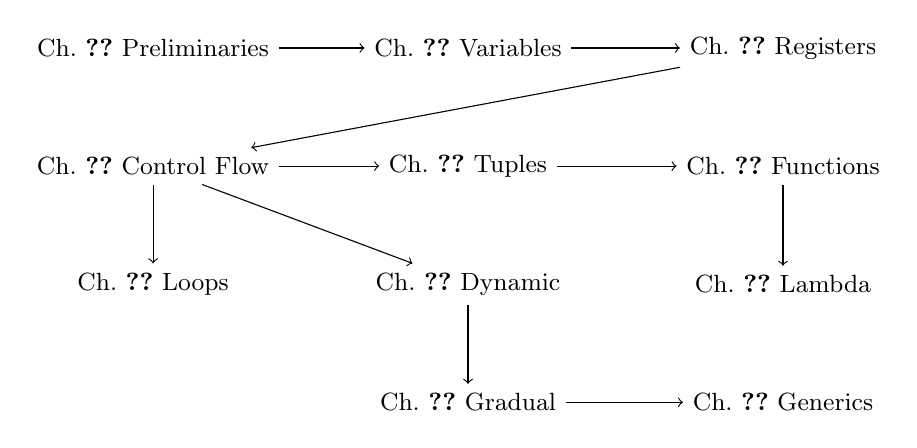
\begin{tikzpicture}[baseline=(current  bounding  box.center)]
  \node (C1) at (0,1.5) {\small Ch.~\ref{ch:trees-recur} Preliminaries};
  \node (C2) at (4,1.5) {\small Ch.~\ref{ch:Rvar} Variables};
  \node (C3) at (8,1.5) {\small Ch.~\ref{ch:register-allocation-Rvar} Registers};
  \node (C4) at (0,0) {\small Ch.~\ref{ch:Rif} Control Flow};
  \node (C5) at (4,0) {\small Ch.~\ref{ch:Rvec} Tuples};
  \node (C6) at (8,0) {\small Ch.~\ref{ch:Rfun} Functions};
  \node (C9) at (0,-1.5) {\small Ch.~\ref{ch:Rwhile} Loops};
  \node (C8) at (4,-1.5) {\small Ch.~\ref{ch:Rdyn} Dynamic};
  \node (C7) at (8,-1.5) {\small Ch.~\ref{ch:Rlam} Lambda};
  \node (C10) at (4,-3) {\small Ch.~\ref{ch:Rgrad} Gradual};
  \node (C11) at (8,-3) {\small Ch.~\ref{ch:Rpoly} Generics};

  \path[->] (C1) edge [above] node {} (C2);
  \path[->] (C2) edge [above] node {} (C3);
  \path[->] (C3) edge [above] node {} (C4);
  \path[->] (C4) edge [above] node {} (C5);
  \path[->] (C5) edge [above] node {} (C6);
  \path[->] (C6) edge [above] node {} (C7);
  \path[->] (C4) edge [above] node {} (C8);
  \path[->] (C4) edge [above] node {} (C9);
  \path[->] (C8) edge [above] node {} (C10);
  \path[->] (C10) edge [above] node {} (C11);
\end{tikzpicture}
  \caption{Diagram of chapter dependencies.}
  \label{fig:chapter-dependences}
\end{figure}

We use the \href{https://racket-lang.org/}{Racket} language both for
the implementation of the compiler and for the input language, so the
reader should be proficient with Racket or Scheme. There are many
excellent resources for learning Scheme and
Racket~\citep{Dybvig:1987aa,Abelson:1996uq,Friedman:1996aa,Felleisen:2001aa,Felleisen:2013aa,Flatt:2014aa}. The
support code for this book is in the \code{github} repository at the
following URL:
\begin{center}\small
  \url{https://github.com/IUCompilerCourse/public-student-support-code}
\end{center}

The compiler targets x86 assembly language~\citep{Intel:2015aa}, so it
is helpful but not necessary for the reader to have taken a computer
systems course~\citep{Bryant:2010aa}. This book introduces the parts
of x86-64 assembly language that are needed.
%
We follow the System V calling
conventions~\citep{Bryant:2005aa,Matz:2013aa}, so the assembly code
that we generate works with the runtime system (written in C) when it
is compiled using the GNU C compiler (\code{gcc}) on Linux and MacOS
operating systems.
%
On the Windows operating system, \code{gcc} uses the Microsoft x64
calling convention~\citep{Microsoft:2018aa,Microsoft:2020aa}. So the
assembly code that we generate does \emph{not} work with the runtime
system on Windows. One workaround is to use a virtual machine with
Linux as the guest operating system.

\section*{Acknowledgments}

The tradition of compiler construction at Indiana University goes back
to research and courses on programming languages by Daniel Friedman in
the 1970's and 1980's.  One of his students, Kent Dybvig, implemented
Chez Scheme~\citep{Dybvig:2006aa}, a production-quality, efficient
compiler for Scheme.  Throughout the 1990's and 2000's, Dybvig taught
the compiler course and continued the development of Chez Scheme.
%
The compiler course evolved to incorporate novel pedagogical ideas
while also including elements of efficient real-world compilers.  One
of Friedman's ideas was to split the compiler into many small
passes. Another idea, called ``the game'', was to test the code
generated by each pass on interpreters.

Dybvig, with help from his students Dipanwita Sarkar and Andrew Keep,
developed infrastructure to support this approach and evolved the
course to use even smaller
nanopasses~\citep{Sarkar:2004fk,Keep:2012aa}.  Many of the compiler
design decisions in this book are inspired by the assignment
descriptions of \citet{Dybvig:2010aa}. In the mid 2000's a student of
Dybvig's named Abdulaziz Ghuloum observed that the front-to-back
organization of the course made it difficult for students to
understand the rationale for the compiler design. Ghuloum proposed the
incremental approach~\citep{Ghuloum:2006bh}.

We thank the many graduate students who served as teaching assistants
for the compiler course at IU. In particular, we thank Andre
Kuhlenschmidt for his work on the garbage collector, Michael Vollmer
for his work on efficient tail calls, and Michael Vitousek for his
help running the first offering of the incremental compiler course at
IU.

We thank Bor-Yuh Chang, John Clements, Jay McCarthy, Joseph Near, Nate
Nystrom, and Michael Wollowski for teaching courses based on early
drafts of this book.

We thank Ronald Garcia for being Jeremy's partner when they took the
compiler course in the early 2000's and especially for finding the bug
that sent the garbage collector on a wild goose chase!

\mbox{}\\
\noindent Jeremy G. Siek \\
Bloomington, Indiana

\mainmatter

%% \part{Environmental Policy Analysis:\break Various Models for Material
%% Flows\break in the Economy}


%% %\begin{partintro}
%% %\partintrotitle{This is an introduction to the part}
%% %Policy analysis may be divided into a number of subspecialities\ldots
%% %
%% %\end{partintro}

%% \chapterauthor{Contributor Name/Names goes here}

%% \chapter[Environmental Policy Analysis with STREAM:\protect\\
%% Equilibrium Model for Material Flows in the Economy]
%% {Environmental Policy Analysis with STREAM: A Partial
%% Equilibrium Model for Material Flows in the Economy}

%% \chaptermark{Environmental Policy Analysis with STREAM}

%% \vspace{-8pt}%
%% \epigraph{What star falls unseen?}{William Faulkner}
%% \epigraph{All seats provide equal viewing of the universe.}{Museum
%% guide, Hayden Planetarium}

%% \endchapepigraph

%% \noindent
%% Robotics has achieved its greatest success to date in the world of industrial manufacturing.
%% Robot arms, or Manipulators, comprise a \$2 billion dollar industry.
%% Bolted at its shoulder to a specific position in the assembly line, the robot arm
%% can move with great speed and accuracy to perform repetitive tasks such as spot
%% welding and painting.

%% \section{Introduction}
%% In the electronics industry, manipulators place
%% surface-mounted components with superhuman precision, making the portable
%% telephone and laptop computer possible.

%% test citation \citet{antibayes} \citep{pijnacker2}

%% \subsection{Test Subsection}
%% Yet for all of their successes, these commercial robots suffer from a fundamental
%% disadvantage: lack of mobility. 

%% \subsubsection{Test subsubsection}
%% A fixed manipulator has a limited range of motion
%% that depends on where it is bolted down. In contrast, a mobile robot would be
%% able to travel throughout the manufacturing plant, flexibly applying its talents
%% wherever it is most effective. 


%% \paragraph{\sansbold{Test paragraph}}
%% For example, AGV (autonomous guided vehicle)
%% robots autono\-mous\-ly deliver parts between various assembly stations
%% by following special electrical guidewires using a custom sensor. The Helpmate
%% service robot transports food and medication throughout hospitals by tracking
%% the position of ceiling lights, which are manually specified to the robot
%% beforehand.\endnote{Several companies have developed autonomous cleaning
%% robots, mainly for large buildings. One such cleaning
%% robot is in use
%% at the Paris Metro. 
%% }

%% The Helpmate service robot transports food and medication throughout hospitals
%% by tracking the position of ceiling lights, which are manually specified to
%% the robot beforehand. Several companies have developed autonomous
%% cleaning robots, mainly for large buildings. 

%% This book focuses on the technology of mobility: how can a mobile robot move
%% unsupervised through real-world environments to fulfill its tasks? The first
%% challenge is locomotion itself. How should a mobile robot move, and what is it
%% about a particular locomotion mechanism that makes it superior to alternative
%% locomotion mechanisms?


%% \subsection{Key Issues for Locomotion}
%% Locomotion is the complement of manipulation. In manipulation, the robot arm
%% is fixed but moves objects in the workspace by imparting force to them. In
%% locomotion, the environment is fixed and the robot moves by imparting force to
%% the environment. In both cases, the scientific basis is the study of actuators that
%% generate interaction forces, and mechinisms that implement disired kinematic
%% and dynamic properties. Locomotion and manipulation thus share the same core
%% issues of stability, contact characteristics, and environmental type:

%% \begin{itemize}
%% \item
%% stability
%% \item
%% number and geometry of contact points
%% \begin{itemize}
%% \item
%% center of gravity
%% \item
%% static/dynamic stability
%% \begin{itemize}
%% \item
%% inclination of terrain
%% \item
%% characteristics of contact
%% \end{itemize}
%% \item
%% contact point/path size and shape
%% \item
%% angle of contact
%% \end{itemize}
%% \item
%% friction
%% \item
%% type of environment
%% \item
%% structure
%% medium (e.g. water, air. soft or hard ground).
%% \end{itemize}
%% For example, Plustech's walking robot provides automatic leg coordination while
%% the human operator chooses an overall direction of travel. Figure
%% 1.5 depicts an underwater vehicle that controls six propellers to autonomously
%% transports food and medication throughout hospitals by tracking the position
%% of ceiling lights, which are manually specified to the robot
%% beforehand.  Several companies have developed autonomous robots.
%% For example, Plustech's walking robot provides automatic leg coordination while
%% the human operator chooses an overall direction of travel. Figure
%% 1.5 depicts an underwater vehicle that controls six propellers to autonomously
%% transports food and medication throughout hospitals by tracking the position
%% of ceiling lights, which are manually specified to the robot
%% beforehand. 


%% \begin{figure}[t]
%% %\centerline{\includegraphics[width=200pt]{figsamp}}
%% \caption[Plustech developed the first application-driven walking robot. It is designed to move
%% wood out of the forest. The leg coordination is automated, but navigation is still done
%% by the human operator on the robot.
%% {\tt http://www.plustech.fi/}]
%% {Plustech developed the first application-driven walking robot. It is designed to move
%% wood out of the forest. The leg coordination is automated, but navigation is still done
%% by the human operator on the robot. {\tt http://www.plustech.fi/}}
%% \end{figure}

%% The six different events are
%% \begin{enumerate}[2.]
%% \item
%% lift right leg
%% \item
%% left let leg
%% \begin{enumerate}[ii.]
%% \item
%% release right leg
%% \item
%% release left leg
%% \begin{enumerate}[(ii)]
%% \item
%% lift both legs together
%% \item
%% release both legs together
%% \end{enumerate}
%% \end{enumerate}
%% \end{enumerate}
%% Of course, this quickly grows quite large. For example, a robot with six legs
%% has far more gaits theoretically.

%% \section{Sample Equations}
%% \begin{equation}
%% \label{eq:rhoCHT}
%% \rho^{\pi}= \frac{RI + \mathbb{E}_{\pi([L,\tau_L]|\textrm{post})}
%% \left[C_L(\taupav+\tau_L) \right]   +
%% \displaystyle{\int_{0}^{P}}{dw~ \mathbb{E}_{\pi_{w_L}}}
%% \Biggl[\/\sum_{n_{L|[\textrm{pre},w]}}C_L(\tau_L)
%% \Biggr]            }      {P +
%% \mathbb{E}_{\pi([L,\tau_L] |\textrm{post})}[\tau_{L}] +\taupav +
%% \displaystyle{ \int_{0}^{P}}{dw~ \mathbb{E}_{\pi_{w_L}}}   
%% \Biggl[\sum_{n_{L|[\textrm{pre},w]}}\tau_L\Biggr]  
%% }
%% \end{equation}
%% As long as
%% $RI - K_LP > 
%% \frac{1}{\beta}$
%% \begin{equation}
%% \left.\begin{array}{lrcl}
%% &\rho^{\pi} &=&  \displaystyle\frac{\beta ( RI + K_L \taupav )-1} {\beta
%% (P+\taupav )}    \\[12pt]
%% \hbox{and}\hbox to .25in{\hfill}&\mathbb{E}[\tau_L | \text{post}]
%% &=&\displaystyle \frac{P+\taupav}{\beta ( RI -
%% K_LP)-1}  
%% \label{eq:analytical_linear}
%% \end{array}\right\}
%% \end{equation} 


%% \subsection{One Leg} 

%% The minimum number of legs a legged robot can have is, of
%% course, one. Minimizing the number of legs is beneficial for several reasons.
%% Body mass is particularly important to walking machines, and the single leg
%% minimizes cumulative leg mass.

%% Omnidirectional locomotion with three spherical wheels The omnidirectional
%% robot depicted in figure 2.23 is based on three spherical wheels, each actuated
%% by one motor. In theis design, the sperical wheels are suspended by three contact
%% points, two given by spherical bearings and one by a wheel connected to
%% the motor axle. This concept provides excellent maneuverability and is simple
%% in design. However, it is limited to flat surfaces and small loads, and it is quite
%% difficult to find round wheels with high friction coefficients.


%% \section{Natbib Citation Mark Up}
%% Citations in the New Math book style are made using the Natbib
%% commands. 

%% \paragraph{\sansbold{Single citations}}
%% may be made using the \verb+\citet+ or \verb+\citep+ command
%% \text{argument}.

%% \blankline

%% \noindent\begin{tabular}{@{}ll}
%% \sansbold{Type}&\sansbold{Results}\\
%% \midrule
%% \verb+\citet{jon90}+&Jones et al. (1990)\\
%% \verb+\citet[chap. 2]{jon90}+&Jones et al. (1990, chap. 2)\\
%%     \verb+\citep{jon90}+	    &   	(Jones et al., 1990)\\
%%     \verb+\citep[chap. 2]{jon90}+ 	&    	(Jones et al., 1990, chap. 2)\\
%%     \verb+\citep[see][]{jon90}+ 	 &    	(see Jones et al., 1990)\\
%%     \verb+\citep[see][chap. 2]{jon90}+ 	&    	(see Jones et al., 1990, chap. 2)\\
%%     \verb+\citet*{jon90}+ 	    &    	Jones, Baker, and Williams (1990)\\
%%     \verb+\citep*{jon90}+	    &    	(Jones, Baker, and Williams,
%%     1990) \\
%% \end{tabular}


%% \paragraph{\sansbold{Multiple citations}}
%% may be made by including more than one citation
%% key in the \verb+\citet+ or \verb+\citep+ command argument.

%% \blankline

%% \noindent\begin{tabular}{@{}ll}
%% \sansbold{Type}&\sansbold{Results}\\
%% \midrule
%% \verb+\citet{jon90,jam91}+&Jones et al. (1990); James et al. (1991)\\
%% \verb+\citep{jon90,jam91}+&(Jones et al., 1990; James et al. 1991)\\
%% \verb+\citep{jon90,jon91}+&(Jones et al., 1990, 1991)\\
%% \verb+\citep{jon90a,jon90b}+&(Jones et al., 1990a,b)\\
%% \end{tabular}

%% \blankline

%% See \url{http://merkel.zoneo.net/Latex/natbib.php}
%% for a reference sheet of natbib commands.

%% \section{Sample Table Note}
%% \begin{table}[h!]
%% \begin{threeparttable}
%% \caption[Time of the transition between Phase 1 and Phase 2]{Time of the transition between Phase 1 and Phase 2\tnote{$a$}
%% \label{tab:label}}\tabfont
%% \setlength{\tabcolsep}{45pt}%
%% \begin{tabular}{@{}ll}
%% \toprule
%%  Run  & Time (min)  \\
%% \midrule
%%   $l1$  & 260   \\
%%   $l2$  & 300   \\
%%   $l3$  & 340   \\
%%   $h1$  & 270   \\
%%   $h2$  & 250   \\
%%   $h3$  & 380   \\
%%   $r1$  & 370   \\
%%   $r2$  & 390   \\
%% \bottomrule
%% \end{tabular}
%% \begin{tablenotes}[flushleft]\footnotesize
%% \item[${a}$]Table note text here.
%% \end{tablenotes}
%% \end{threeparttable}
%% \end{table}

%% \chapter{Gravitational Waves}

%% \section{Mass in Spacetime}
%% As objects with
%% mass move around in spacetime,\endnote{Test for endnote for endnote for endnote for endnote for endnote for endnote for endnote for endnote for endnote for endnote} the curvature changes to reflect the
%% changed locations of those objects. In certain circumstances,
%% accelerating objects generate changes in this curvature, which
%% propagate outwards at the speed of light in a wave-like manner. These
%% propagating phenomena are known as gravitational waves.\endnote{Prof. Gabriela Gonz\'alez, from Louisiana State University,
%% said: ``We have discovered gravitational waves from the merger of black
%% holes. It's been a very long road, but this is just the beginning.
%% }

%% \subsection{Gauss's Law for Gravity}
%% In physics, \sfbfit{Gauss's law for gravity}, also known
%% as \sfbfit{Gauss's flux
%% theorem for}\break \sfbfit{gravity}, is a law of physics that is essentially
%% equivalent to Newton's law of universal gravitation. It is named after
%% Carl Friedrich Gauss.\index{authors}{Gauss, Carl Friedrich}

%% The gravitational field \boldmath$g$\unboldmath (also called gravitational acceleration) is
%% a vector field---a vector at each point of space (and time). It is
%% defined so that the gravitational force experienced by a particle is
%% equal to the mass of the particle multiplied by the gravitational
%% field at that point.

%% Gravitational flux is a surface integral of the gravitational field
%% over a closed surface, analogous to how magnetic flux is a surface
%% integral of the magnetic field.

%% As a result of the divergence theorem, a host of physical laws can be
%% written in both a differential form (where one quantity is the
%% divergence of another) and an integral form (where the flux of one
%% quantity through a closed surface is equal to another quantity).
%% Three examples are Gauss's law (in electrostatics), Gauss's law for
%% magnetism, and Gauss's law for gravity.     
%% Gauss's law for gravity states:
%% \begin{theorem}
%%     The gravitational flux through any closed surface is proportional
%%     to the enclosed mass.  \end{theorem}
%% \begin{proof}
%% The integral form of Gauss's law is:
%% \[ \oiint
%% \mathbf {E} \cdot \mathrm {d} \mathbf {A}  = 
%% {\frac {Q}{\varepsilon _{0}}}  \]
%% for any closed surface $S$ containing charge $Q$. By the divergence
%% theorem, this equation is equivalent to:
%% \[
%% \iiint\limits_{V}
%%  \boldnabla \cdot \mathbf{E} \,\, \mathrm{d}   V={\frac
%% {Q}{\varepsilon _{0}}}
%% \]
%% for any volume $V$ containing charge $Q$. By the relation between charge
%% and charge density, this equation is equivalent to:
%% \[\iiint\limits_{V} \boldnabla \cdot\mathbf{E}\,\,\mathrm{d} V = 
%% \iiint
%% \limits _{V}{\frac {\rho }{\varepsilon _{0}}}\ \mathrm {d} V\]
%% for any volume $V$. In order for this equation to be simultaneously
%% true for every possible volume $V$,  
%% it is necessary (and sufficient) for the integrands to be equal
%% everywhere.  Therefore, this equation is equivalent to:
%% \[    \boldnabla \cdot\mathbf{E} = \frac{\rho }{\varepsilon _{0}}. \]
%% Thus the integral and differential forms are equivalent.
%% \end{proof}


%% \subsection{Gravitational Waves}

%% Gravitational waves are `ripples' in the fabric of space-time caused
%% by some of the most violent and energetic processes in the Universe.
%% Albert Einstein predicted the existence of gravitational waves in 1916
%% in his general theory of relativity. Einstein's mathematics showed
%% that massive accelerating objects (such as neutron stars or black
%% holes orbiting each other) would disrupt space-time in such a way that
%% `waves' of distorted space would radiate from the source (like the
%% movement of waves away from a stone thrown into a pond). Furthermore,
%% these ripples would travel at the speed of light through the Universe,
%% carrying with them information about their cataclysmic origins, as
%% well as invaluable clues to the nature of gravity itself.

%% %\begin{notation}
%% %$g_{\mu\nu}(x^\lambda)=g_{\nu\mu}(x^\lambda)$&symmetric tensor\\
%% %$g_{\mu\nu}\equiv\eta_{\mu\nu}=\mathrm{diag}(−1,1,1,1)$&Minkowski
%% %spacetime\\
%% %\end{notation}
%% The strongest gravitational waves are produced by catastrophic events
%% such as colliding black holes, the collapse of stellar cores
%% (supernovae), coalescing neutron stars or white dwarf stars, the
%% slightly wobbly rotation of neutron stars that are not perfect
%% spheres, and the remnants of gravitational radiation created by the
%% birth of the Universe itself.\endnote{``Gravitational waves go through everything. They are hardly affected
%% by what they pass through, and that means that they are perfect
%% messengers,'' said Prof Bernard Schutz, from Cardiff University, UK.
%% \index{authors}{Schutz, Bernard}

%% \begin{quote}
%% The information carried on the gravitational wave is exactly the same
%% as when the system sent it out; and that is unusual in astronomy. We
%% can't see light from whole regions of our own galaxy because of the
%% dust that is in the way, and we can't see the early part of the Big
%% Bang because the Universe was opaque to light earlier than a certain
%% time.

%% With gravitational waves, we do expect eventually to see the Big Bang
%% itself, he told the BBC.
%% \end{quote}

%% In addition, the study of gravitational waves may ultimately help
%% scientists in their quest to solve some of the biggest problems in
%% physics, such as the unification of forces, linking quantum theory
%% with gravity.}

%% \begin{extract}
%% (Kostas D. Kokkotas, Article for the Encyclopedia of Physical Science
%% and Technology, 3rd Edition, Volume 7, Academic Press, (2002))\\
%% The distance $ds$ between two neighboring events, one with coordinates
%% $x^\mu$ and the other with coordinates $x^\mu + \mathrm
%% {dx}^\mu+ \mathrm{dx}^\mu$, can be expressed as a function of the coordinates via a
%% symmetric tensor $g_{\mu\nu}(x^\lambda)=g_{\nu\mu}(x^\lambda)$, i.e.,
%% %% \begin{equation}
%% %% \mathrm{ds}^2=g_{\mu\nu}\,\mathrm{dx}^μ\,\mathrm{dx}^\nu
%% %% \end{equation}
%% This is a generalization of the standard measure of distance between two points in
%% Euclidian space. For the Minkowski spacetime (the spacetime of special relativity),
%% %$g_{\mu\nu}\equiv\eta_{\mu\nu}=\mathrm{diag}(−1,1,1,1)$.
%% \end{extract}

%% Though\index{authors}{Kokkotas, Kostas} gravitational waves were predicted to exist in 1916, actual
%% proof of their existence wouldn't arrive until 1974, 20 years after
%% Einstein's death.
%% Since then, many astronomers have studied the timing of pulsar radio
%% emissions and found similar effects, further confirming the existence
%% of gravitational waves. But these confirmations had always come
%% indirectly or mathematically and not through actual `physical'
%% contact.

%% That was the case up until September 14, 2015, when LIGO, for the
%% first time, physically sensed distortions in spacetime itself caused
%% by passing gravitational waves generated by two colliding black holes
%% nearly 1.3 billion light years away! LIGO and its discovery will go
%% down in history as one of the greatest human scientific achievements.

%% \section*{A Dialogue}

%% From the NY Times article of February 11, 2016,
%% {\it Gravitational Waves Detected, Confirming Einstein's Theory}\/:

%% \begin{dialogue}
%% \speaker{Francis C\'ordova}
%% It’s been decades, through a lot of different technological
%% innovations,
%% [and the foundation’s advisory board had] really scratched their heads on this one.

%% \speaker{Janna Levin}I was freaking out!

%% \speaker{Robert Garisto} [the editor of Physical Review Letters] 
%% I got goose bumps while reading the LIGO paper.
%% \end{dialogue}

%% \noindent The discovery is a great triumph for three physicists---Kip Thorne of
%% the California Institute of Technology, Rainer Weiss of the
%% Massachusetts Institute of Technology and Ronald Drever, formerly of
%% Caltech and now retired in Scotland---who bet their careers on the
%% dream of measuring the most ineffable of Einstein’s notions.
%% \index{authors}{C\'ordova, Francis}
%% \index{authors}{Levin, Janna}
%% \index{authors}{Garisto, Robert}
%% \index{authors}{Thorne, Kip}
%% \index{authors}{Weiss, Rainer}
%% \index{authors}{Drever, Ronald}

%% \begin{extract}
%% Gravitational waves are not sound waves, and the
%% general public easily could have been led to that conclusion. Sound
%% waves travel only through a medium such as air; ripples in spacetime
%% don’t need any medium to support them. Sound waves propagate at the
%% speed of sound; gravitational waves move at the speed of light. Even
%% someone with superhuman hearing could never listen in on a black hole
%% collision.

%% So why the connection between sound and gravitational waves? 
%% \begin{itemize}
%% \item LIGO detects gravitational waves with frequencies
%% between several hertz and several kilohertz, the sweet spot for human
%% hearing. 
%% \item When two stellar-mass black holes collide, they happen to
%% jiggle spacetime at the same frequency as that of pressure waves in
%% the air that our ears pick up as sound.     
%% \end{itemize}
%% The LIGO discovery proves that black hole binaries exist, and that
%% those binaries can merge within the age of the universe.
%% \end{extract}

%% While the origins of gravitational waves
%% can be extremely violent, by the time the waves reach the Earth they
%% are millions of times smaller and less disruptive. In fact, by the
%% time gravitational waves from the first detection reached LIGO, the
%% amount of space-time wobbling they generated was thousands of times
%% smaller than the nucleus of an atom! Such inconceivably small
%% measurements are what LIGO was designed to make.


%% \begin{description}
%% \item[Wave passes]
%% As a gravitational wave passes an observer, that observer will find
%% spacetime distorted by the effects of strain. 

%% \item[Distances]
%% Distances between
%% objects increase and decrease rhythmically as the wave passes, at a
%% frequency corresponding to that of the wave. 
%% \end{description}
%% This occurs despite such
%% free objects never being subjected to an unbalanced force. The
%% magnitude of this effect decreases proportional to the inverse
%% distance from the source.

%% Such systems cannot be observed with more
%% traditional means such as optical telescopes or radio telescopes, and
%% so gravitational-wave astronomy gives new insights into the working of
%% the Universe. In particular, gravitational waves could be of interest
%% to cosmologists as they offer a possible way of observing the very
%% early Universe. This is not possible with conventional astronomy,
%% since before recombination the Universe was opaque to electromagnetic
%% radiation.

%% Precise measurements of gravitational waves will also
%% allow scientists to more thoroughly test the general theory of
%% relativity.

%% \begin{boxedtext}{Frank Wilczek on Einstein and Gravitation}
%% Einstein's general relativity, as a theory of gravitation, is so tight
%% conceptually that it allows only two free parameters: Newton’s
%% constant and the cosmological term. It has passed every test that
%% physicists and astronomers have devised. Yet there are reasons to
%% remain dissatisfied.

%% \section{First}
%% First, the strength of gravity is grossly disproportionate to the
%% strength of other forces. If we believe in the unity of nature’s
%% operating system, how can that be? 

%% \subsection{Second}
%% Second, the measured value of the
%% mass density of space devoid of matter---the cosmological term, often
%% called dark energy---is incommensurate with reasonable expectations. Why
%% is it much smaller than theory suggests, yet not zero? 

%% \subsubsection{Third}
%% Third, the
%% equations that follow from straightforward quantization of general
%% relativity break down in extreme conditions. What are the
%% consequences? Those issues are important agenda items for the next 100
%% years of physics. In the boxes, I've indicated a promising way to
%% approach the question of the weakness of gravity. Here I'll offer a
%% few comments on the other issues.


%% \begin{extract}
%% Theorists have estimated several contributions to the cosmological
%% term-positive and negative---whose individual absolute values far exceed
%% the observed total value. Thus the term’s observed smallness indicates
%% delicate cancellations that our core theories do not explain. Perhaps,
%% as suggested by Steven Weinberg, the explanation is anthropic. Too
%% large a cosmological term would lead the universe to expand so rapidly
%% that formation of structure in the universe would be inhibited.
%% Neither galaxies nor stars nor planets would form, and thus observers
%% could not emerge. Is that anthropic argument the best physics can
%% do---is resistance futile? Or is some deeper principle at work?
%% \end{extract}

%% \section*{Conceptual difficulty}
%% The conceptual difficulty of reconciling our theory of gravity,
%% general relativity, with the principles of quantum mechanics has been
%% the subject of much hyperbole. I think it is important, therefore,
%% first to bring it down to earth.   

%% (Frank Wilczek, Physics Today, April 2016,
%% \url{scitation.aip.org/content/aip/magazine/physicstoday/article/69/4/10.1063/PT.3.3137})
%% \end{boxedtext}
%% \index{authors}{Wilczek, Frank}

%% In principle, gravitational waves could exist at any frequency.
%% However, very low frequency waves would be impossible to detect and
%% there is no credible source for detectable waves of very high
%% frequency. Stephen Hawking and Werner Israel list different frequency
%% bands for gravitational waves that could plausibly be detected,
%% ranging from 10--7 Hz up to 1011 Hz. 

%% In theory, the loss of energy through gravitational radiation could
%% eventually drop the Earth into the Sun. However, the total energy of
%% the Earth orbiting the Sun (kinetic energy + gravitational potential
%% energy) is about 1.14$\times$1036 joules of which only 200 joules per second
%% is lost through gravitational radiation, leading to a decay in the
%% orbit by about $1\times10$--15 meters per day or roughly the diameter of a
%% proton. At this rate, it would take the Earth approximately $1\times 1013$
%% times more than the current age of the Universe to spiral onto the
%% Sun. This estimate overlooks the decrease in r over time, but the
%% majority of the time the bodies are far apart and only radiating
%% slowly, so the difference is unimportant in this example.

%% \begin{table}
%% \caption{A table of acceleration equations.}\tabfont
%% \begin{tabular}{@{}l|l}    
%% \toprule
%% \it With initial velocity&\it Starting from rest\\
%% \midrule
%% $v_f=v_i+ a \Delta\, t$&$v_f=a\Delta\, t$\\
%% $\Delta\, d=v_i \Delta\, t + 1/2 a \Delta\, t^2$&
%% $\Delta\, d= 1/2 a \Delta\, t^2$\\
%% $v_f=\sqrt{v_i^2+2a\Delta\, d}$&
%% $v_f=\sqrt{2a\Delta\, d}$\\
%% \bottomrule
%% \end{tabular}
%% \end{table}

%% More generally, the rate of orbital decay can be approximated by [32].
%% \[
%%     \frac{\mathrm{d}r}{\mathrm{d}t} = - \frac{64}{5}\,
%%     \frac{G^3}{c^5}\, \frac{(m_1m_2)(m_1+m_2)}{r^3}\ ,  
%% \]
%% where $r$ is the separation between the bodies, $t$ time, G Newton's
%% constant, $c$ the speed of light, and $m1$ and $m2$ the masses of the
%% bodies. This leads to an expected time to merger of 
%% \begin{equation}
%%     t= \frac{5}{256}\, \frac{c^5}{G^3}\,
%%     \frac{r^4}{(m_1m_2)(m_1+m_2)}.  
%% \end{equation}
%% For example a pair of solar mass neutron stars in a circular orbit at
%% a separation of $1.89\times108$ $m$ (189,000 km) has an orbital
%% period of 1,000 


%% \begin{boxedtext}{Two Theorems and a Corollary}
 	
%% \begin{theorem}[Birkhoff's Theorem]
%% The metric of the Schwarzschild black hole is the unique spherically
%% symmetric solution of the vacuum {\it Einstein field equations}.
%% \[G^{\mu\nu}=0.\]

%% Stated another way, a spherically symmetric gravitational field in
%% empty space must be static, with a metric given by the Schwarzschild
%% black hole\index{authors}{Swarzchild, Karl}
%% \index{authors}{Birkhoff, George David}
%%  metric.
%% \end{theorem}

%% \begin{corollary}
%% A corollary states that the metric inside a spherical cavity inside a
%% spherical mass distribution is the Minkowski metric. 
%% \end{corollary}

%% \begin{theorem}[Schwarzschild Black Hole]
%%  A black hole with zero charge $Q = 0$ and no angular momentum $J = 0$.
%% The exterior solution for such a black hole is known as the
%% Schwarzschild solution (or Schwarzschild metric), and is an exact
%% unique solution to the Einstein field equations of general relativity
%% for the general static isotropic metric (i.e., the most general metric
%% tensor that can represent a static isotropic gravitational field), 
%% \[
%% d\tau^2=B(r)dt^2 - A(r)dr^2-r^2 \sin^2\theta\, d\phi^2.
%% \]
%% \end{theorem}

%% \vspace{-6pt}

%% \noindent
%% In 1915, when Einstein first proposed them, the 
%% Einstein field equations appeared so complicated that he did not 
%% believe that a solution would ever be found. 
%% He was therefore quite surprised when, only a year later, 
%% Karl Schwarzschild  (1916) discovered one by making the assumption of
%% spherical symmetry. 
%% \end{boxedtext}



%% \section{Samples of Programming Code}

%% \begin{verbatim}
%% procedure bubbleSort( A : list of sortable items )
%%     n = length(A)
%%     repeat
%%        newn = 0
%%        for i = 1 to n-1 inclusive do
%%           if A[i-1] > A[i] then
%%              swap(A[i-1], A[i])
%%              newn = i
%%           end if
%%        end for
%%        n = newn
%%     until n = 0
%% end procedure
%% \end{verbatim}

%% \newpage

%% \noindent
%% Algorithm environment:


%% %% \begin{algorithm} takes option [p][b][t][h],  or some combination, like \begin{figure}
%% \begin{algorithm}[h]
%% \caption{A sample in an algorithm environment.}
%% \begin{algorithmic}
%% \If {$i\geq maxval$}
%%     \State $i\gets 0$
%% \Else
%%     \If {$i+k\leq maxval$}
%%         \State $i\gets i+k$
%%     \EndIf
%% \EndIf
%% \end{algorithmic}
%% \end{algorithm}

%% \begin{boxedtext}{Two Examples  of Programming Code}

%% \vspace{-1\topsep}

%% \begin{verbatim}
%% procedure bubbleSort( A : list of sortable items )
%%     n = length(A)
%%     repeat
%% \end{verbatim}
%% \end{boxedtext}

%% \begin{exercises}
%% \exer{For Hooker's data, Exercise 1.2, use the Box and Cox and Atkinson procedures to determine a appropriate transformation of PRES
%% in the regression of PRES on TEMP. find $\hat\lambda$, $\tilde\lambda$,
%% the score test, and the added variable plot for the score. 
%% Summarize the results.}

%% \subexer{The following data were collected in a study of the effect of dissolved sulfur
%% on the surface tension of liquid copper (Baes and Killogg, 1953).}

%% \medskip

%% \hspace{3.5pt}\begin{tabular}{r@{}lcc}
%% \toprule
%% &&\multicolumn2c{$Y$= Decrease in Surface Tension}\\
%% \multicolumn2c{$x$ = Weight \% sulfur}
%% &\multicolumn2c{(dynes/cm), two Replicates}\\
%% \midrule
%% 0.&034&301&316\\
%% 0.&093&430&422\\
%% 011.&30&593&586\\
%% \bottomrule
%% \end{tabular}


%% \subexer{Find the transformations of $X$ and $Y$ sot that in the transformed scale 
%% the regression is linear.}

%% \subexer{Assuming that $X$ is transformed to $\ln(X)$, which choice of $Y$ gives 
%% better results,
%% $Y$ or $\ln(Y)$? (Sclove, 1972).}

%% \sidebysidesubsubexer{In the case of $\Delta_1$?}{In the case of $\Delta_2$?}

%% \exer{Examine the Longley data, Problem 3.3, for applicability of assumptions of the
%% linear model.}

%% \sidebysidesubexer{In the case of $\Gamma_1$?}{In the case of $\Gamma_2$?}
%% \[
%%     t= \frac{5}{256}\, \frac{c^5}{G^3}\,
%%     \frac{r^4}{(m_1m_2)(m_1+m_2)}.  
%% \]

%% \end{exercises}

%% \begin{chapappendix}[Chapter Appendix: Dark Matter Is Not Composed of Black Holes]

%% \section{The Canada France Hawaii Lensing Survey}

%% Did you know that less than 4\% of our Universe is made up of regular
%% matter - the type that makes up the Earth, the planets and the stars?
%% The rest is 'dark' and invisible, but we know that it is there through
%% its effects on the regular matter that we can see. The gravity of Dark
%% Matter causes galaxies to clump together in a giant cosmic web, and
%% Dark Energy is pushing space itself apart at an accelerated rate. With
%% some of the world's best telescopes we can directly witness the
%% ongoing battle between these two strange entities.

%% \subsection{CFHTL}
%% The Canada-France-Hawaii Telescope Lensing Survey uses an innovative
%% technique called gravitational lensing to observe the invisible dark
%% matter in our Universe. Using data accumulated over five years by the
%% CFHT Legacy Survey, the CFHTLenS team have analysed the images of over
%% 10 million galaxies. The light emitted by these galaxies has taken
%% nearly half the age of the Universe to reach us and has been bent and
%% distorted by the massive clumps of dark matter it has passed by.
%% Exploiting this fact that `mass bends light', as predicted by
%% Einstein, we have privileged access to the mysterious components of
%% the Universe that cannot otherwise be observed.

%% \section{Dark Matter and Black Holes}
%% We know that dark matter exists because of our mathematical graphs of
%% how fast the material in a galaxy is rotating in relation to the
%% center of the galaxy (where most of the galactic material is located).
%% And as a result of these graphs, we know that dark matter surrounds
%% galaxies. In the end, the farther out you go, the more mass
%% grows\ldots and
%% it grows by a lot. So in short, we know that dark matter isn’t just
%% some black hole that exists out in the middle of intergalactic space
%% based on the way that galaxies rotate and evolve over time.

%%  As Emma Grocutt, from the
%% CFHTL Survey notes:\index{authors}{Grocutt, Emma}

%% \begin{extract}
%% The most interesting thing about dark matter is not simply that we
%% can't see it, it's that we know dark matter is not made of the same
%% stuff as normal baryonic matter. This is actually why we can't see
%% it---baryons interact with each other through gravity, nuclear forces and
%% the electrostatic force. These interactions are what allow baryonic
%% matter (such as stars) to emit light, and what prevent you from
%% putting your hand through a table---the particles of your hand are
%% electrostatically repelled from the particles in the table. Dark
%% matter, however, only interacts through gravity. This is why we see
%% its effects on the motions of galaxies and stars, but why we can't see
%% it directly; it does not emit or absorb light. Dark matter particles
%% can also pass through regular matter almost completely undetected
%% since they don't interact electrostatically, meaning we can't touch it
%% or sense it in any direct way.
%% \end{extract}

%% \end{chapappendix}

%% \setcounter{chapter}{2}

%% \clearpage

\appendix

%% \chapter{Evaluating the Significance of the Proof of Gravity
%% Waves} 

%% \section{On a Par with Determination of Structure of DNA}


%% Prof Karsten Danzmann, from the Max Planck Institute for
%% \index{authors}{Danzmann, Karsten}
%% \index{subject}{Max Planck Institute for Gravitational Physics}
%% Gravitational Physics and Leibniz University in Hannover, Germany, is
%% a European leader on the collaboration.\footnote{Text and graphics
%% from
%% \url{http://www.bbc.com/news/science-environment-35524440}}

%% He said the detection was one of the most important developments in
%% science since the discovery of the Higgs particle, and on a par with
%% the determination of the structure of DNA.
%% \index{subject}{Nobel Prize}

%% \begin{figure}[h!]
%% %\centerline{\includegraphics[width=\textwidth]{gravwaves}}
%% \vspace{2pt}
%% \caption{Graphic showing two black holes generating gravity waves.}
%% \end{figure}

%% ``It is the first ever direct detection of gravitational waves; it's
%% the first ever direct detection of black holes and it is a
%% confirmation of General Relativity because the property of these black
%% holes agrees exactly with what Einstein predicted almost exactly 100
%% years ago.''\index{authors}{Einstein, Albert}
%% \index{subject}{Albert Einstein!General Relativity}
%% \begin{equation}
%% d\tau^2=B(r)dt^2 - A(r)dr^2-r^2 \sin^2\theta\, d\phi^2.
%% \end{equation}

%% \begin{sidewaysfigure}
%% %\includegraphics[width=\textheight]{gravwaves}
%% \vspace{-11pt}
%% \caption{Graphic showing two black holes generating gravity waves.
%% (rotated figure)}
%% \end{sidewaysfigure}

%% \begin{sidewaystable}
%% \begin{center}
%% \begin{threeparttable}
%% \caption{More relevant tabular information.\label{tbl-2}}\tabfont
%% \begin{tabular}{@{}lrrrrrrrrrrr}
%% \toprule
%% Star & Height & $d_{x}$ & $d_{y}$ & $n$ & $\chi^2$ & $R_{maj}$ & $R_{min}$ &
%% \multicolumn{1}{c}{$P^a$} & $P R_{maj}$ & $P R_{min}$ &
%% \multicolumn{1}{c}{$\Theta^b$} \\
%% \midrule
%% 1 &33472.5 &-0.1 &0.4  &53 &27.4 &2.065  &1.940 &3.900 &68.3 &116.2 &-27.639\\
%% 2 &27802.4 &-0.3 &-0.2 &60 &3.7  &1.628  &1.510 &2.156 &6.8  &7.5 &-26.764\\
%% 3 &29210.6 &0.9  &0.3  &60 &3.4  &1.622  &1.551 &2.159 &6.7  &7.3 &-40.272\\
%% 4 &32733.8 &-1.2\rlap{\tnote{$c$}} &-0.5 &41 &54.8 &2.282  &2.156 &4.313 &117.4 &78.2 &-35.847\\
%% 5 & 9607.4 &-0.4 &-0.4 &60 &1.4  &1.669\rlap{\tnote{$c$}} &1.574 &2.343 &8.0  &8.9 &-33.417\\
%% 6 &31638.6 &1.6  &0.1  &39 &315.2 & 3.433 &3.075 &7.488 &92.1 &25.3 &-12.052\\
%% \bottomrule
%% \end{tabular}
%% \begin{tablenotes}[flushleft]\footnotesize
%% \item[$a$]Sample footnote for table~\ref{tbl-2} that was
%% generated with the \LaTeX\ table environment
%% \item[$b$]Yet another sample footnote for table
%% \ref{tbl-2}
%% \item[$c$]Another sample footnote for
%% table~\ref{tbl-2}
%% \end{tablenotes}
%% \end{threeparttable}
%% \end{center}
%% \end{sidewaystable}


%% \section{Ripples in the Fabric of Space-Time}

%% \begin{itemize}
%% \item
%%     Gravitational waves are a prediction of the Theory of General
%%     Relativity 
%% \item
%%     Their existence has been inferred by science but only now
%%     directly detected 
%% \item
%%     They are ripples in the fabric of space and time produced by
%%     violent events 
%% \item
%%     Accelerating masses will produce waves that propagate at the
%%     speed of light 
%% \item
%%     Detectable sources ought to include merging black holes and
%%     neutron stars 
%% \item
%%     Ligo fires lasers into long, L-shaped tunnels; the waves disturb
%%     the light 
%% \item
%%     Detecting the waves opens up the Universe to completely new
%%     investigations 
%% \end{itemize}


%% \subsection{Stephen Hawking Agrees on Importance}
%% That view was reinforced by Prof Stephen Hawking, who is an expert on
%% black holes.\footnote{Perhaps somewhat immodestly, 
%% this claim is made
%% on Hawking's website (\url{www.hawking.org.uk}):
%% ``Stephen Hawking is regarded as one of the
%% most brilliant theoretical  physicists since Einstein.''
%% Though, of course, it may well be true!}
%% Speaking exclusively to BBC News, he said he believed
%% that the detection marked a key moment in scientific history.\endnote{Stephen Hawking said that the detection of gravity waves
%% marked a key moment in scientific history.}
%% \index{authors}{Hawking, Stephen}

%% ``Gravitational waves provide a completely new way at looking at the
%% Universe. The ability to detect them has the potential to
%% revolutionise astronomy. This discovery is the first detection of a
%% black hole binary system and the first observation of black holes
%% merging,'' he said.

%% ``Apart from testing (Albert Einstein's theory of) General Relativity,
%% we could hope to see black holes through the history of the Universe.
%% We may even see relics of the very early Universe during the Big Bang
%% at some of the most extreme energies possible.''
%% \index{authors}{Albert Einstein}

%% \subsection{Too Beautiful to Be True?}
%% We found a beautiful signature of the merger of two black holes and
%% it agrees exactly - fantastically\nobreak - with the numerical solutions to
%% Einstein equations\ldots it looked too beautiful to be true," said Prof
%% Danzmann.\index{subject}{beauty}\index{subject}{truth}\index{subject}{truth and
%% beauty!truth}\index{subject}{beauty and truth!beauty}

\backmatter

%% \addtocontents{toc}{\vspace{11pt}}

%% \begin{glossary}
%% \term{Absolute Zero}{
%% The lowest temperature possible, equivalent to -273.15$^{\deg}$C (or
%% 0$^{\deg}$ on the
%% absolute Kelvin scale), at which point atoms cease to move altogether
%% and molecular energy is minimal. The idea that it is impossible,
%% through any physical process, to lower the temperature of a system to
%% zero is known as the Third Law of Thermodynamics.}
%% \index{subject}{Absolute zero}
%% \index{subject}{Third Law of Thermodynamics}

%% \term{Alpha Particle (Alpha Decay)}{A particle of 2 protons and 2 neutrons (essentially a helium nucleus)
%% that is emitted by an unstable radioactive nucleus during radioactive
%% decay. It is a relatively low-penetration particle due its
%% comparatively low energy and high mass.}
%% \index{subject}{Alpha Particle}

%% \term{Angular Momentum}{A measure of the momentum of a body in rotational
%% motion about its centre of mass. Technically, the angular momentum of
%% a body is equal to the mass of the body multiplied by the cross
%% product of the position vector of the particle with its velocity
%% vector. The angular momentum of a system is the sum of the angular
%% momenta of its constituent particles, and this total is conserved
%% unless acted on by an outside force.}

%% \term{Anthropic Principle}
%% {The idea that the fundamental constants of physics and chemistry are
%% just right (or ``fine-tuned'') to allow the universe and life as we know
%% it to exist, and indeed that the universe is only as it is because we
%% are here to observe it. Thus, we find ourselves in the kind of
%% universe, and on the kind of planet, where conditions are ripe for our
%% form of life.}

%% \term{Antimatter}{Pair production and pair annihilation
%% of hydrogen and antihydrogen particles. 
%% A large
%% accumulation of antiparticles---antiprotons, antineutrons and
%% positrons (antielectrons)---which have opposite properties to normal
%% particles (e.g. electrical charge), and which can come together to
%% make antiatoms. When matter and antimatter meet, they self-destruct in
%% a burst of high-energy photons or gamma rays. The laws of physics seem
%% to predict a pretty much 50/50 mix of matter and antimatter, despite
%% the observable universe apparently consisting almost entirely of
%% matter, known as the ``baryon asymmetry problem.''}
%% \index{subject}{antimatter}
%% \index{subject}{antimatter, definition of}
%% \index{subject}{baryon asymmetry problem}

%% \end{glossary}

%% \begin{endbookexercises}
%% \exer{For Hooker's data, Exercise 1.2, use the Box and Cox and Atkinson procedures to determine a appropriate transformation of PRES
%% in the regression of PRES on TEMP. find $\hat\lambda$, $\tilde\lambda$,
%% the score test, and the added variable plot for the score. 
%% Summarize the results.}

%% \subexer{The following data were collected in a study of the effect of dissolved sulfur
%% on the surface tension of liquid copper (Baes and Killogg, 1953).}

%% \hspace{3.5pt}\begin{tabular}{rlcc}
%% \toprule
%% &&\multicolumn2c{$Y$= Decrease in Surface Tension}\\
%% \multicolumn2c{$x$ = Weight \% sulfur}
%% &\multicolumn2c{(dynes/cm), two Replicates}\\
%% \midrule
%% 0.&034&301&316\\
%% 0.&093&430&422\\
%% 0.&30&593&586\\
%% \bottomrule
%% \end{tabular}

%% \subexer{Find the transformations of $X$ and $Y$ sot that in the transformed scale 
%% the regression is linear.}

%% \subexer{Assuming that $X$ is transformed to $\ln(X)$, which choice of $Y$ gives 
%% better results,
%% $Y$ or $\ln(Y)$? (Sclove, 1972).}

%% \sidebysidesubsubexer{In the case of $\Delta_1$?}{In the case of $\Delta_2$?}

%% \exer{Examine the Longley data, Problem 3.3, for applicability of assumptions of the
%% linear model.}

%% \sidebysidesubexer{In the case of $\Gamma_1$?}{In the case of $\Gamma_2$?}

%% \[
%%     t= \frac{5}{256}\, \frac{c^5}{G^3}\,
%%     \frac{r^4}{(m_1m_2)(m_1+m_2)}.  
%% \]

%% \end{endbookexercises}

%% \theendnotes

%% \nocite{*} is a way to get all the entries in the .bib file to print in the bibliography:
\nocite{*}\let\bibname\refname
\addcontentsline{toc}{fmbm}{\refname}
\printbibliography

%% \begin{contributors}[twocolumn]

%% \contrib 
%% Professor Alan Guth\\
%% Center for Theoretical Physics\\
%% Massachusetts Institute of Technology\\
%% Cambridge, Massachusetts, USA

%% \contrib 
%% Professor Andrei Linde\\
%% Department of Physics\\
%% Stanford University\\
%% Stanford, CA, USA
%% \end{contributors}

 \printindex{authors}{Author Index}
 \printindex{subject}{Subject Index}


\end{document}

